% Created 2023-10-17 mar. 13:18
% Intended LaTeX compiler: pdflatex

% =================================BASE====================================%
\documentclass[10pt]{article}
\usepackage[left=2cm,right=2cm,top=2cm,bottom=2cm]{geometry} % Marges
\usepackage[T1]{fontenc} % Nécessaire avec FrenchBabel
\usepackage[utf8]{inputenc} % Important pour symboles Francophones, é,à,etc


% Calligraphie
\usepackage{lmodern}
\renewcommand{\familydefault}{cmr} % La meilleure police (CMU Serif Roman) (Je me suis battu).
\usepackage{mathrsfs} %Permet la command \mathscr (Lettres attachées genre)

% Bibliographie
\usepackage[round, sort]{natbib} % Bibliographie
\bibliographystyle{abbrvnat}


\usepackage{amsmath, amssymb, amsthm} % Symb. math. (Mathmode+Textmode) + Beaux théorèmes.
\usepackage{mathtools,cancel,xfrac} % Utilisation de boîtes \boxed{} + \cancelto{}{}
\usepackage{graphicx, wrapfig} % Géstion des figures.
\usepackage{hyperref} % Permettre l'utilisation d'hyperliens.
\usepackage{color} % Permettre l'utilisation des couleurs.
\usepackage[dvipsnames]{xcolor} % Couleurs avancées.
\usepackage{titling} % Donne accès à \theauthor, \thetitle, \thedate

% Physique
\usepackage{physics} % Meilleur package pour physicien. 
\usepackage{pxfonts} % Rajoute PLEIN de symboles mathématiques, dont les intégrales doubles et triples

% Style
\usepackage{lipsum} % For fun
\usepackage{tikz} % Realisation de figures TIKZ.
\usepackage{empheq} % Boite autour de MULTIPLE équations

% Français
\usepackage[french]{babel} % Environnements en Français.
% ==============================BASE-(END)=================================%



% ================================SETTINGS=================================%
% Pas d'indentation en début de paragraphe :
\setlength\parindent{0pt}
\setlength{\parskip}{0.15cm}

% Couleurs de hyperliens :
\definecolor{mypink}{RGB}{147, 0, 255}
\hypersetup{colorlinks, 
             filecolor=mypink,
             urlcolor=mypink, 
             citecolor=mypink, 
             linkcolor=mypink, 
             anchorcolor=mypink}

% Numéros d'équations suivent les sections :
\numberwithin{equation}{section} 

% Les « captions » sont en italique et largeur limitée
\usepackage[textfont = it]{caption} 
\captionsetup[wrapfigure]{margin=0.5cm}

% Retirer le l'écriture en gras dans la table des matières
\usepackage{tocloft}
\renewcommand{\cftsecfont}{\normalfont}
\renewcommand{\cftsecpagefont}{\normalfont}

% Change bullet style
\usepackage{pifont}
\usepackage{enumitem}
%\setlist[itemize,1]{label=\ding{224}}
\setlist[itemize,1]{label=\ding{239}}
\renewcommand{\boxtimes}{\blacksquare}
% ================================SETTINGS=================================%



% ==============================NEWCOMMANDS================================%

% Vecteurs de base :
\newcommand{\nvf}{\vb{\hat{n}}}
\newcommand{\ivf}{\vb{\hat{i}}}
\newcommand{\jvf}{\vb{\hat{j}}}
\newcommand{\kvf}{\vb{\hat{k}}}
\newcommand{\uu}{\vb*{u}}
\newcommand{\vv}{\vb*{v}}

% Physics empty spaces 
\newcommand{\typical}{\vphantom{A}}
\newcommand{\tall}{\vphantom{A^{x^x}_p}}
\newcommand{\grande}{\vphantom{\frac{1}{xx}}}
\newcommand{\venti}{\vphantom{\sum_x^x}}
\newcommand{\pt}{\hspace{1pt}} % One horizontal pt space

% Moyenne numérique entre deux points de grilles. 
\newcommand{\xmean}[1]{\overline{#1}^x}
\newcommand{\ymean}[1]{\overline{#1}^y}
\newcommand{\zmean}[1]{\overline{#1}^z}
\newcommand{\xymean}[1]{\overline{#1}^{xy}}

% Tilde over psi
\newcommand{\tpsi}{\tilde{\psi}}
\newcommand{\tphi}{\tilde{\phi}}

% Nota Bene env : (\ding{89})
\newcommand{\nb}{\raisebox{0.8pt}{\scriptsize\textleaf}\ $\mathscr{N. B.}$\hspace{4pt}}
   
% ==============================NEWCOMMANDS================================%



% ==============================PAGE-TITRE=================================%
% Titlepage 
\newcommand{\mytitlepage}{
\begin{titlepage}
\begin{center}
{\Large Contrat Été 2023 \par}
\vspace{2cm}
{\Large \MakeUppercase{\thetitle} \par}
\vspace{2cm}
RÉALISÉ DANS LE CADRE\\ D'UN PROJET POUR \par
\vspace{2cm}
{\Large ISMER--UQAR \par}
\vspace{2cm}
{\thedate}
\end{center}
\vfill
Rédaction \\
{\theauthor}\\
\url{charles-edouard.lizotte@uqar.ca}\\
ISMER-UQAR
\end{titlepage}
}
% ==============================PAGE-TITRE=================================%



% =================================ENTÊTE==================================%
\usepackage{fancyhdr}
\pagestyle{fancy}
\setlength{\headheight}{13pt}
\renewcommand{\headrulewidth}{0.025pt} % Ligne horizontale en haut

\fancyhead[R]{\textit{\thetitle}}
\fancyhead[L]{\ \thepage}
\fancyfoot[R]{\textit{\theauthor}}
\fancyfoot[L]{}
\fancyfoot[C]{} 
% =================================ENTÊTE==================================%
\author{Charles-Édouard Lizotte}
\date{20/10/2023}
\title{Carnet de bord, Université McGill}
\hypersetup{
 pdfauthor={Charles-Édouard Lizotte},
 pdftitle={Carnet de bord, Université McGill},
 pdfkeywords={},
 pdfsubject={},
 pdfcreator={Emacs 28.2 (Org mode 9.6.5)}, 
 pdflang={French}}
\begin{document}

\mytitlepage
\tableofcontents\newpage
\section{Debuggage et implémentation transfert de masse -- \textit{<2023-10-16 lun.>}}
\label{sec:org5937cc8}
\subsection{Vérifier que ce n'est pas un problème de viscosité -- \textit{<2023-10-16 lun.>}}
\label{sec:org3357d4d}
\label{orgf05ef60}
DEADLINE: \textit{<2023-10-17 mar.>}
Avant tout, David a remarqué que les champs de vorticité (\(\zeta_k\)) étaient extrêmement bruités, ce qui signifie qu'il y a clairement un manque à gagner en terme de viscosité.
Une viscosité plus forte permet essentiellement de se débarrasser des fluctuations aux plus petites échelles.
N'oublions pas que nous sommes passées d'une viscosité au 4ème degré vers une viscosité au second degré quand nous cherchions le problème au bord, il y a quelques semaines.
Tout ça vient confirmer ma théorie de l'escalier.\bigskip

En sommes, de nouveaux test ont été effectuées pour le schéma de viscosité exprimé par
\begin{equation}
   \vb{D} = Ah_2 \cdot \laplacian{\uu} - Ah_4\cdot \gradient^4\uu.
\end{equation}
En ce mardi matin, les résultats sont exprimés dans le tableau \ref{tab:org601b00e}.



\begin{table}[htbp]
\caption{\label{tab:org601b00e}Résumé des expériences réalisées dans le but de retrouver la bonne viscosité.}
\centering
\begin{tabular}{c|c|c|c|l}
\hline
Ah\textsubscript{2} & Ah\textsubscript{4} & dx & min(\sfrac{$L_d$}{dx}) & Nombre d'itér.\\[0pt]
[ -- ] & [ -- ] & [ km ] & [ -- ] & [ -- ]\\[0pt]
\hline
\hline
0.0 & (1\texttimes{}10\textsuperscript{-5})\pt\texttimes{} dx\textsuperscript{4} & 3.9 & 5.363 & 736 272 (Active)\\[0pt]
0.0 & (2\texttimes{}10\textsuperscript{-5})\pt\texttimes{} dx\textsuperscript{4} & 3.9 & 5.363 & 736 272 (Active)\\[0pt]
0.0 & (5\texttimes{}10\textsuperscript{-5})\pt\texttimes{} dx\textsuperscript{4} & 3.9 & 5.363 & 113\\[0pt]
0.0 & (1\texttimes{}10\textsuperscript{-4})\pt\texttimes{} dx\textsuperscript{4} & 3.9 & 5.363 & 48\\[0pt]
0.0 & (5\texttimes{}10\textsuperscript{-4})\pt\texttimes{} dx\textsuperscript{4} & 3.9 & 5.363 & 23\\[0pt]
\hline
\hline
\end{tabular}
\end{table}


Pour conclure, il semble que tous nos problèmes venaient bel et bien du changement de viscosité que nous avions appliqué pour régler le problème d'ondes de Kelvin aux bord (problème qui a été réglé \href{rapport-2023-10-06.pdf}{il y a deux rapports}).
Comme on peut l'observer à la figure \ref{fig:org0b377de}, les \emph{eddies} sont maintenant très \emph{smooth} et non-bruités -- ce qui contraste fortement avec le dernier schéma de viscosité où l'on utilisait une viscosité au deuxième ordre plutôt qu'un viscosité avec un Laplacien d'ordre 4.
Ce qu'il faut retenir de cela c'est que le schéma utilisé dans l'article de \Citet{chen_2021} était robuste.
Vaut mieux ne pas trop s'en éloigner. 

\begin{figure}[htbp]
\centering
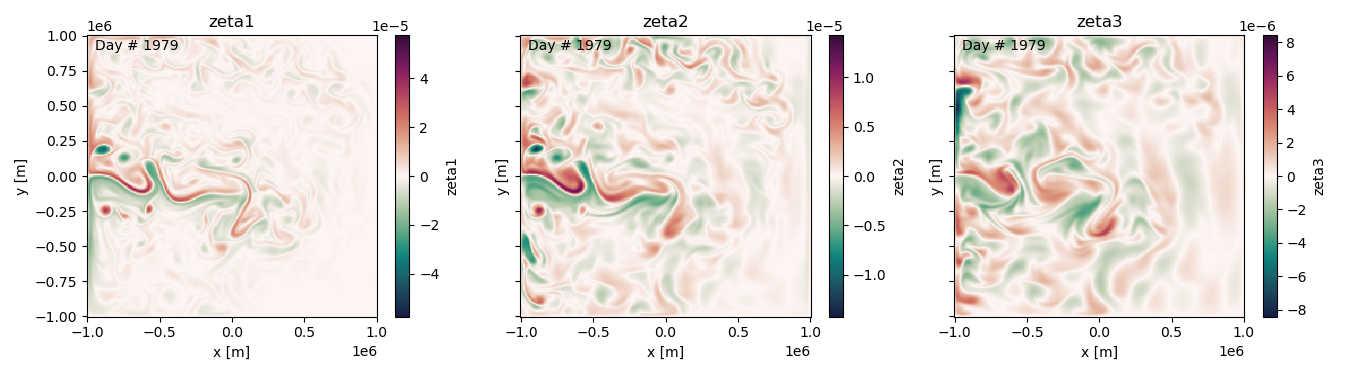
\includegraphics[width=.9\linewidth]{figures/debuggage/2023_10_17_smooth_zeta.png}
\caption{\label{fig:org0b377de}Vorticité dans les trois couches après 1900 jours pour le modèle « shallow water ». On observe que les tourbillons sont très lisses dans la promière couche, en opposition au précédent schéma de viscosité utilisé.}
\end{figure}


\subsection{« Stencil » de transfert de masse}
\label{sec:orge2cf174}
Louis-Philippe propose d'utiliser un stencil à 21 points pour redistribuer la masse (Voir figure \ref{orge64b552}).
En gros, on en retirerait sur le point fautif pour rejouter du \emph{h} aux points des alentours, ce qui en fait une redistribution horizontale de la masse.\bigskip

\nb Pour l'instant, je met tout ça sur la glace, car la solution trouvée à la section \ref{orgf05ef60} semble suffisante.
Si la solution proposée à la prochaine section n'est pas suffisante, nous reviendrons sur le transfert de masse avec notre \emph{stencil}. 

\begin{figure}[!h]
\centering
\begin{tikzpicture}
   \fill [blue!5] (1,0) -- (4,0) -- (4,1) -- (5,1) -- (5,4) -- (4,4) -- (4,5) -- (1,5) -- (1,4) -- (0,4) -- (0,1) -- (1,1) -- (1,0);
   \fill [blue!12] (1,1) rectangle (4,4);
   \draw [dotted,thin] (1,0) grid (4,5);
   \draw [dotted,thin] (0,1) grid (5,4);
   \draw [] (1,0) -- (4,0) -- (4,1) -- (5,1) -- (5,4) -- (4,4) -- (4,5) -- (1,5) -- (1,4) -- (0,4) -- (0,1) -- (1,1) -- (1,0);
   \fill [cyan!50] (2,2) rectangle (3,3); 
   \draw [] (2,2) rectangle (3,3);
   %
   \draw (2.5,2.5) node {+1};
\end{tikzpicture}
\caption{\label{orge64b552}Stencil de redistribution de la masse.}
\end{figure}

\section{Solution à la dérive de Stokes -- \textit{<2023-10-16 lun.>}}
\label{sec:org1b8958e}
Grossièrement, il est sorti deux possibilités pour régler le problème des petites échelles qui sortent de Wavewatch :
\begin{itemize}
\item Il serait possible de diminuer la résolution de Wavewatch et de réinterpoler les points de courants à l'aide de la méthose employée dans la figure \ref{orgc5e9c70}.

\begin{figure}[h!]
\begin{center}
\begin{tikzpicture}
% Big grid
\fill [blue!5] (0,0) rectangle (3,3);
\fill [blue!5] (3,3) rectangle (6,6);
% Grid
\draw (0,0) rectangle (6,6) ;
\draw [dotted] (0,0) grid (6,6) ;
\draw [step=3.0] (0,0) grid (6,6) ;
% Carré
\draw [cyan, thick] (2,2) rectangle (5,5) ;
\fill [cyan!50, opacity=0.5] (3,3) rectangle (4,4);
% Coordinates 
\foreach \x in {1,2,3}
\foreach \y in {1,2,3}
{\draw (\x-0.5,\y-0.5) node [] {1,1};}
%
\foreach \x in {4,5,6}
\foreach \y in {1,2,3}
{\draw (\x-0.5,\y-0.5) node [] {2,1};}
%
\foreach \x in {1,2,3}
\foreach \y in {4,5,6}
{\draw (\x-0.5,\y-0.5) node [] {1,2};}
%
\foreach \x in {4,5,6}
\foreach \y in {4,5,6}
{\draw (\x-0.5,\y-0.5) node [] {2,2};}
% Axis:
\foreach \y in {1,2,3,4,5,6} {\draw (-0.5,\y-0.5) node [cyan] {\y};}
\foreach \x in {1,2,3,4,5,6} {\draw (\x-0.5,-0.5) node [cyan] {\x};}
%
\end{tikzpicture}
\end{center}
\begin{equation}
   {\color{cyan}u(4,4)} = \qty(\sfrac{1}{9})\cdot u(1,1) + \qty(\sfrac{2}{9})\cdot u(2,1) + \qty(\sfrac{2}{9})\cdot u(1,2) + \qty(\sfrac{4}{9})\cdot u(2,2).
\end{equation}
\caption{\label{orgc5e9c70}« Stencil » utilisé pour obtenir le champs aux plus grandes échelles.}
\end{figure}
\end{itemize}




\bibliography{/aos/home/celizotte/Desktop/Documentation/master-bibliography}
\end{document}